\documentclass[12pt]{article}
\usepackage{amsmath, amssymb}
\usepackage{graphicx}
\usepackage{enumitem}
\usepackage[margin=1in]{geometry}

\begin{document}

\begin{center}
    {\LARGE \bf GATE -MT 2023}\\[1em]
    ai25btech11009 \quad Dasu Harshith Kumar
\end{center}

\begin{enumerate}

\item “You are delaying the completion of the task. Send  ----- contributions at the earliest.”  (GATE -MT 2023)
 \begin{enumerate}[label=(\alph*)]
  \item you are
  \item your
  \item you’re
  \item yore
 \end{enumerate}

\item References : ------ : : Guidelines : Implement (By word meaning) (GATE -MT 2023)
\begin{enumerate}[label=(\alph*)]
  \item Sight
  \item Site
  \item Cite
  \item Plagiarise
\end{enumerate}

\item In the given figure, PQRS is a parallelogram with PS = 7 cm, PT = 4 cm and PV = 5 cm. What is the length of RS in cm? (The diagram is representative.) (GATE -MT 2023)
\begin{enumerate}[label=(\alph*)]
  \item \(\frac{20}{7}\)
  \item \(\frac{28}{5}\)
  \item \(\frac{9}{2}\)
  \item \(\frac{35}{4}\)
\end{enumerate}


\begin{center}
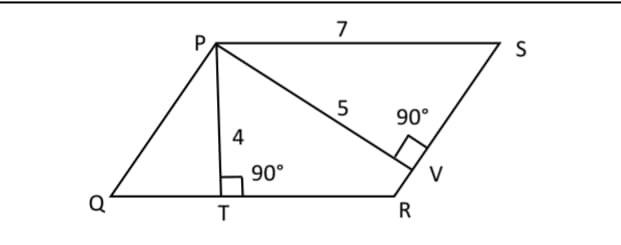
\includegraphics[width=0.5\textwidth]{images/qqq3i.jpg}
\end{center}

\item In 2022, June Huh was awarded the Fields medal, which is the highest prize in Mathematics.
When he was younger, he was also a poet. He did not win any medals in the International Mathematics Olympiads. He dropped out of college.
Based only on the above information, which one of the following statements can be logically inferred with certainty? (GATE -MT 2023)
\begin{enumerate}[label=(\alph*)]
  \item Every Fields medalist has won a medal in an International Mathematics Olympiad.
  \item Everyone who has dropped out of college has won the Fields medal.
  \item All Fields medalists are part-time poets.
  \item Some Fields medalists have dropped out of college.
\end{enumerate}

\item A line of symmetry is defined as a line that divides a figure into two parts in a way such that each part is a mirror image of the other part about that line.
The given figure consists of 16 unit squares arranged as shown. In addition to the three black squares, what is the minimum number of squares that must be coloured black, such that both PQ and MN form lines of symmetry? (The figure is representative) (GATE -MT 2023)
\begin{enumerate}[label=(\alph*)]
  \item 3
  \item 4
  \item 5
  \item 6
\end{enumerate}


\begin{center}
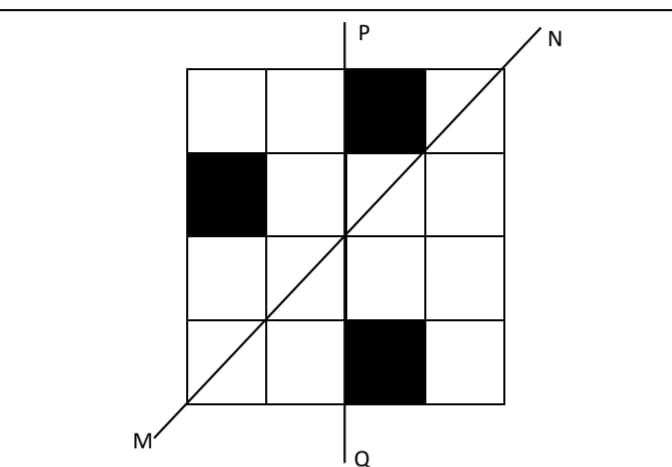
\includegraphics[width=0.4\textwidth]{images/qqq5i.jpg}
\end{center}

\item Human beings are one among many creatures that inhabit an imagined world. In this imagined world, some creatures are cruel. If in this imagined world, it is given that the statement “Some human beings are not cruel creatures” is FALSE, then which of the following set of statement(s) can be logically inferred with certainty? (GATE -MT 2023)
(i) All human beings are cruel creatures.
(ii) Some human beings are cruel creatures.
(iii) Some creatures that are cruel are human beings.
(iv) No human beings are cruel creatures.
\begin{enumerate}[label=(\alph*)]
  \item only (i)
  \item only (iii) and (iv)
  \item only (i) and (ii)
  \item (i), (ii) and (iii)
\end{enumerate}

\item To construct a wall, sand and cement are mixed in the ratio of 3:1. The cost of sand and that of cement are in the ratio of 1:2.  
If the total cost of sand and cement to construct the wall is 1000 rupees, then what is the cost (in rupees) of cement used? (GATE -MT 2023)
\begin{enumerate}[label=(\alph*)]
  \item 400
  \item 600
  \item 800
  \item 200
\end{enumerate}

\item The World Bank has declared that it does not plan to offer new financing to Sri Lanka, which is battling its worst economic crisis in decades, until the country has an adequate macroeconomic policy framework in place. In a statement, the World Bank said Sri Lanka needed to adopt structural reforms that focus on economic stabilisation and tackle the root causes of its crisis. The latter has starved it of foreign exchange and led to shortages of food, fuel, and medicines. The bank is repurposing resources under existing loans to help alleviate shortages of essential items such as medicine, cooking gas, fertiliser, meals for children, and cash for vulnerable households.
Based only on the above passage, which one of the following statements can be inferred with certainty? (GATE -MT 2023)
\begin{enumerate}[label=(\alph*)]
  \item According to the World Bank, the root cause of Sri Lanka’s economic crisis is that it does not have enough foreign exchange.
  \item The World Bank has stated that it will advise the Sri Lankan government about how to tackle the root causes of its economic crisis.
  \item According to the World Bank, Sri Lanka does not yet have an adequate macroeconomic policy framework.
  \item The World Bank has stated that it will provide Sri Lanka with additional funds for essentials such as food, fuel, and medicines.
\end{enumerate}

\item The coefficient of \(x^4\) in the polynomial \((x-1)^3 (x-2)^3\) is equal to ------.  (GATE -MT 2023)
\begin{enumerate}[label=(\alph*)]
  \item 33
  \item -3
  \item 30
  \item 21
\end{enumerate}

\item Which one of the following shapes can be used to tile (completely cover by repeating) a flat plane, extending to infinity in all directions, without leaving any empty spaces in between them? The copies of the shape used to tile are identical and are not allowed to overlap. (GATE -MT 2023)
\begin{enumerate}[label=(\alph*)]
  \item circle
  \item regular octagon
  \item regular pentagon
  \item rhombus
\end{enumerate}

\item At one atmosphere pressure, \(\alpha\)-Fe transforms to \(\gamma\)-Fe above 912 °C. Density of \(\gamma\)-Fe is more than that of \(\alpha\)-Fe. Choose the correct statement.  (GATE -MT 2023)
\begin{enumerate}[label=(\alph*)]
  \item Increasing the pressure above one atmosphere lowers the \(\alpha\)-Fe to \(\gamma\)-Fe transformation temperature.
  \item Increasing the pressure above one atmosphere raises the \(\alpha\)-Fe to \(\gamma\)-Fe transformation temperature.
  \item Molar volume of \(\gamma\)-Fe is higher than the molar volume of \(\alpha\)-Fe.
  \item Pressure change will not have any effect on the \(\alpha\)-Fe to \(\gamma\)-Fe transformation temperature.
\end{enumerate}

\item Formation of an ideal solution leads to  (GATE -MT 2023)
\begin{enumerate}[label=(\alph*)]
  \item increase in entropy
  \item decrease in volume
  \item increase in enthalpy
  \item decrease in entropy
\end{enumerate}

\item Order (O) and degree (D) of the differential equation \(\left(\frac{dy}{dx}\right)^3 = \sqrt{\frac{d^2y}{dx^2}} + 10\) are  (GATE -MT 2023)
\begin{enumerate}[label=(\alph*)]
  \item \(O = 2\) and \(D=1\)
  \item \(O = 1\) and \(D=2\)
  \item \(O = 6\) and \(D=1\)
  \item \(O = 2\) and \(D=6\)
\end{enumerate}

\item At one atmosphere pressure, iron (Fe) and nickel (Ni) oxidize as  
\[
2Fe + O_2 \leftrightarrow 2FeO \quad \Delta G^0 = -527400 + 128 T \text{ J} \\
2Ni + O_2 \leftrightarrow 2NiO \quad \Delta G^0 = -471200 + 172 T \text{ J}
\]
Identify the correct statement. Given: Temperature \(T\) in Kelvin. (GATE -MT 2023)
\begin{enumerate}[label=(\alph*)]
  \item Fe can reduce NiO at all temperatures
  \item Fe can reduce NiO only above 1000 K
  \item Ni can reduce FeO at all temperatures
  \item Ni can reduce FeO only above 1000 K
\end{enumerate}

\item For laminar fluid flow through a smooth circular tube, the relation between friction factor (\(f\)) and Reynolds number (Re) is (GATE -MT 2023)
\begin{enumerate}[label=(\alph*)]
  \item \(f = \frac{16}{Re}\)
  \item \(f = \frac{24}{Re}\)
  \item \(f = \frac{16}{\sqrt{Re}}\)
  \item \(f = \frac{24}{\sqrt{Re}}\)
\end{enumerate}

\item Among the following options, a process for liquid-liquid separation is (GATE -MT 2023)
\begin{enumerate}[label=(\alph*)]
  \item Smelting
  \item Roasting
  \item Sintering
  \item Calcination
\end{enumerate}

\item The most effective concentration step for sulfide ores is (GATE -MT 2023)
\begin{enumerate}[label=(\alph*)]
  \item Froth flotation
  \item Magnetic separation
  \item Gravity separation
  \item Electrostatic separation
\end{enumerate}

\item The gas distribution in a blast furnace is controlled by the shape of
\begin{enumerate}[label=(\alph*)] (GATE -MT 2023)
  \item Cohesive zone
  \item Deadman zone
  \item Raceway zone
  \item Chemical reserve zone
\end{enumerate}

\item Diamond has low  (GATE -MT 2023)
\begin{enumerate}[label=(\alph*)]
  \item electrical conductivity
  \item modulus of elasticity
  \item hardness
  \item thermal conductivity
\end{enumerate}

\item For self-diffusion in polycrystalline copper with a lattice diffusion coefficient \(D_L\), grain boundary diffusion coefficient \(D_{GB}\), and surface diffusion coefficient \(D_S\), the correct relationship is  (GATE -MT 2023)
\begin{enumerate}[label=(\alph*)]
  \item \(D_S > D_{GB} > D_L\)
  \item \(D_L > D_S > D_{GB}\)
  \item \(D_{GB} > D_S > D_L\)
  \item \(D_{GB} = D_S = D_L\)
\end{enumerate}

\item Magnitude of Burgers vector of the dislocation resulting from reaction of dislocations with Burgers vectors \(\frac{a}{2}[101]\) and \(\frac{a}{2}[0\bar{1}\bar{1}]\) is  (GATE -MT 2023)
\begin{enumerate}[label=(\alph*)]
  \item \(\frac{a}{\sqrt{2}}\)
  \item \(\sqrt{2} a\)
  \item \(\frac{a}{2}\)
  \item \(2 a\)
\end{enumerate}

\item The mechanism of creep for a single crystal as depicted in the schematic is  (GATE -MT 2023)
\begin{enumerate}[label=(\alph*)]
  \item Nabarro-Herring creep
  \item Grain boundary sliding
  \item Dislocation creep
  \item Coble creep
\end{enumerate}

\item The value of \(\lim_{x \to 1} \frac{7x^7 - 20 x^5 + 13 x}{3 x^3 + x - 4}\) is  (GATE -MT 2023)
\begin{enumerate}[label=(\alph*)]
  \item \(-\frac{38}{10}\)
  \item \(-\frac{51}{10}\)
  \item \(\frac{38}{10}\)
  \item undefined
\end{enumerate}

\item Match the defects in Column I with corresponding metal forming techniques in Column II.  (GATE -MT 2023)

\begin{center}
\begin{tabular}{ll}
Column I & Column II \\
(P) Cold shut & (1) Rolling \\
(Q) Zipper breaks & (2) Sheet metal forming \\
(R) Stretcher strains & (3) Drawing \\
(S) Center burst & (4) Forging \\
\end{tabular}
\end{center}

\begin{enumerate}[label=(\alph*)]
  \item P – 4, Q – 1, R – 2, S – 3
  \item P – 4, Q – 2, R – 3, S – 1
  \item P – 1, Q – 4, R – 2, S – 3
  \item P – 3, Q – 1, R – 4, S – 2
\end{enumerate}

\item In rolling, the point on the surface of contact between roll and sheet where surface velocity of the roll is equal to velocity of the sheet is referred as  (GATE -MT 2023)
\begin{enumerate}[label=(\alph*)]
  \item no-slip point
  \item no-stick point
  \item maximum slip point
  \item maximum stick point
\end{enumerate}












\item When cracks propagate in a brittle material, the following option(s) is/are correct:
\begin{enumerate}[label=(\alph*)]
\item elastic strain energy decreases
\item surface energy increases
\item surface energy decreases
\item elastic strain energy increases
\end{enumerate}

\item Which of the following is/are responsible for reducing the high cycle fatigue life of a component?
\begin{enumerate}[label=(\alph*)]
\item increasing the mean stress at constant amplitude
\item increasing the surface roughness
\item employing shot peening
\item absence of sharp corners in the component
\end{enumerate}

\item The non-destructive testing technique(s) for detecting internal defects in a steel component is/are:
\begin{enumerate}[label=(\alph*)]
\item X-ray tomography
\item Ultrasonic technique
\item Gamma radiography
\item Dye penetrant technique
\end{enumerate}

\item The condition(s) for high degree of mutual substitutional solid solubility for two metals is/are:
\begin{enumerate}[label=(\alph*)]
\item metals should have same valence
\item metals should have same crystal structure
\item the difference in atomic size of metals should be less than 15\%
\item the difference in electronegativity of metals should be large
\end{enumerate}

\item The sum of eigenvalues of the matrix
\[
\begin{bmatrix}
4 & 3 & 2 \\
0 & -1 & 2 \\
0 & 0 & -3
\end{bmatrix}
\]
is \underline{\hspace{2cm}} (integer).

\item The probability of setting an easy exam paper by three setters are \(\frac{1}{2}\), \(\frac{1}{3}\), and \(\frac{1}{4}\). If all three are setting one paper each, then the probability that at least one of the papers will be easy is \underline{\hspace{2cm}} (round off to 2 decimal places).

\item Maximum number of phases that can be in equilibrium for a 5-component system at constant temperature and pressure is \underline{\hspace{2cm}} (integer).

\item A liquid of density 900 kg/m\(^3\) is flowing over a flat plate with a free stream velocity of 0.1 m/s. The laminar boundary layer thickness at a distance of 0.2 m from the leading edge of the plate is 0.007 m. The viscosity of the liquid in centipoise is \underline{\hspace{2cm}} (round off to 2 decimal places).

\item The rate constant of a reaction at 400 K is three times the value at 300 K. The activation energy of the reaction in kJ mol\(^{-1}\) is \underline{\hspace{2cm}} (round off to 1 decimal place).  
Given: Universal gas constant, R = 8.314 J mol\(^{-1}\) K\(^{-1}\).

\item The maximum value of function \(f(x) = 4x^3 - 24x^2 + 36\) in the domain \([-1,5]\) is \underline{\hspace{2cm}} (round off to nearest integer).

\item Taking \(S\) as entropy, \(T\) as temperature, \(P\) as pressure, and \(V\) as volume, match Column I with Column II:

\begin{center}
\begin{tabular}{ll}
Column I & Column II \\
(A) Gibbs Free Energy & (1) depends on T, V and composition \\
(B) Helmholtz Free Energy & (2) depends on T, P and composition \\
(C) Enthalpy & (3) depends on S, P and composition \\
(D) Internal Energy & (4) depends on S, V and composition \\
\end{tabular}
\end{center}

Options:  
\begin{enumerate}[label=(\alph*)]
\item A – 2, B – 1, C – 3, D – 4
\item A – 4, B – 3, C – 2, D – 1
\item A – 3, B – 1, C – 4, D – 2
\item A – 2, B – 1, C – 4, D – 3
\end{enumerate}

\item Match the transport processes in Column I with the relationships in Column II:

\begin{center}
\begin{tabular}{ll}
Column I & Column II \\
(P) Molecular momentum transport & (1) Stefan-Boltzmann law \\
(Q) Molecular mass transport & (2) Newton’s law of viscosity \\
(R) Molecular energy transport & (3) Fick’s law \\
(S) Radiation energy transport & (4) Fourier law \\
\end{tabular}
\end{center}

Options:  
\begin{enumerate}[label=(\alph*)]
\item P – 2, Q – 3, R – 4, S – 1
\item P – 4, Q – 3, R – 2, S – 1
\item P – 3, Q – 1, R – 4, S – 2
\item P – 2, Q – 1, R – 4, S – 3
\end{enumerate}

\item For supersonic O\(_2\) jet in basic oxygen furnace steelmaking, choose the correct combination from the following:

(1) Converging-diverging nozzle  
(2) Diverging-converging nozzle  
(3) O\(_2\) velocity greater than sound velocity at nozzle throat (Mach number > 1)  
(4) O\(_2\) velocity equal to sound velocity at nozzle throat (Mach number = 1)  
(5) Exit O\(_2\) jet pressure ≥ atmospheric pressure  
(6) Exit O\(_2\) jet pressure < atmospheric pressure  

Options:  
\begin{enumerate}[label=(\alph*)]
\item (1), (4), (5)
\item (1), (3), (6)
\item (2), (3), (5)
\item (2), (4), (5)
\end{enumerate}

\item Elutriator is used to separate particles based on their sizes in flowing air as shown in the figure.

Assuming spherical particles, the diameter (\(D_{50}\)) of the suspended particles which have 50\% chance to report to overflow by turbulent air flow is expressed as

\begin{enumerate}[label=(\alph*)]
\item \(D_{50} = \frac{3 f v^2 \rho_a}{4 g (\rho_s - \rho_a)}\)
\item \(D_{50} = \left(\frac{18 \mu v}{g f (\rho_s - \rho_a)}\right)^{0.5}\)
\item \(D_{50} = \left(\frac{9 \mu v}{2 g (\rho_s - \rho_a)}\right)^2\)
\item \(D_{50} = \frac{3 f v \rho_a}{8 g (\rho_s - \rho_a)}\)
\end{enumerate}































\item A fluid flow field is given by the velocity vector \(\vec{V} = e^{xyz}(x \hat{i} + z \hat{k})\). The curl of velocity at (1, 2, 3) is
\begin{enumerate}[label=(\alph*)]
\item \(e^{6}(9 \hat{i} - 16 \hat{j} - 3 \hat{k})\)
\item \(e^{6}(9 \hat{i} - 3 \hat{k})\)
\item \(e^{6}(9 \hat{i} + 16 \hat{j} - 3 \hat{k})\)
\item \(e^{6}(-16 \hat{i} + 9 \hat{j} - 3 \hat{k})\)
\end{enumerate}

\item Given \(\vec{\phi} = xy \hat{i} + yz \hat{j} + xz \hat{k}\), \(S\) is a surface bounded by planes \(x=0, y=0, z=0, x=3, y=2, z=1\). If \(\hat{n}\) is the unit vector normal to \(S\), then \(\iint_S \vec{\phi} \cdot \hat{n}\, dS\) is
\begin{enumerate}[label=(\alph*)]
\item 18
\item 9
\item 36
\item 3
\end{enumerate}

\item Match the processes in Column I with the corresponding applications in Column II.
\[
\begin{array}{ll}
\textbf{Column I} & \textbf{Column II} \\
(P) \text{Fused salt electrolysis} & (1) \text{Ironmaking} \\
(Q) \text{Carbothermal reduction} & (2) \text{Aluminium extraction} \\
(R) \text{Oxidation-refining} & (3) \text{Copper extraction} \\
(S) \text{Matte converting} & (4) \text{Steelmaking} \\
\end{array}
\]

\begin{enumerate}[label=(\alph*)]
\item P – 2, Q – 1, R – 4, S – 3
\item P – 4, Q – 3, R – 2, S – 1
\item P – 3, Q – 1, R – 4, S – 2
\item P – 2, Q – 4, R – 1, S – 3
\end{enumerate}

\item Match Column I with Column II.
\[
\begin{array}{ll}
\textbf{Column I} & \textbf{Column II} \\
(P) \text{Gallium arsenide} & (1) \text{Superconductor} \\
(Q) \text{Barium titanate} & (2) \text{Soft magnetic material} \\
(R) \text{Iron - 4 wt.\% silicon} & (3) \text{Semiconductor} \\
(S) \text{Yttrium-barium-copper oxide} & (4) \text{Piezoelectric material} \\
\end{array}
\]

\begin{enumerate}[label=(\alph*)]
\item P – 3, Q – 4, R – 2, S – 1
\item P – 2, Q – 4, R – 3, S – 1
\item P – 3, Q – 2, R – 1, S – 4
\item P – 4, Q – 2, R – 1, S – 3
\end{enumerate}

\item Match the plots in Section I with the corresponding functions in Section II.

\textbf{Section I}
\begin{center}
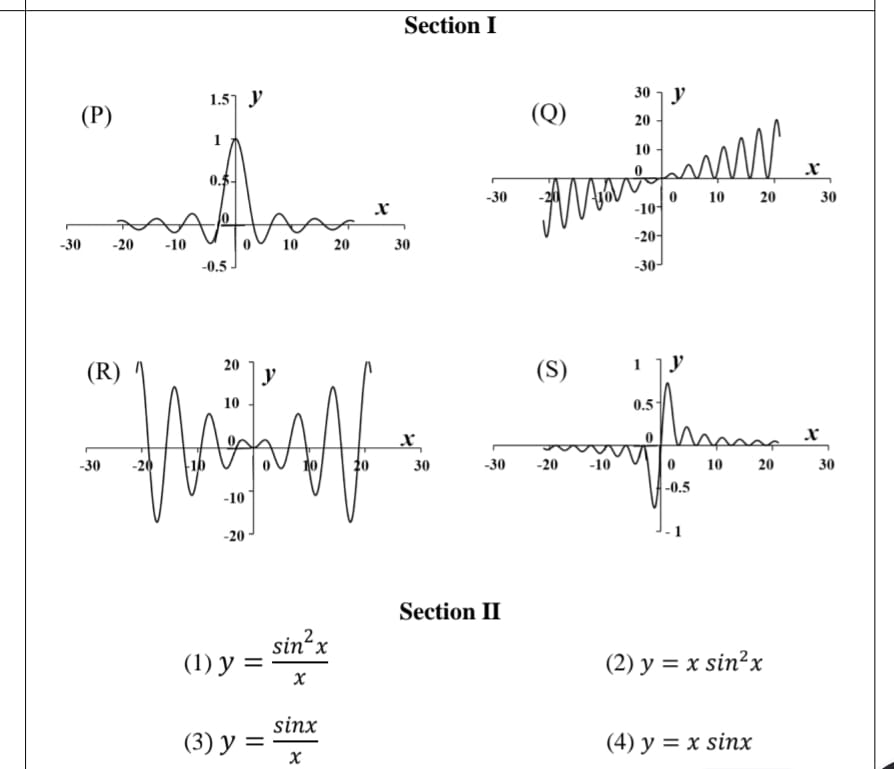
\includegraphics[width=0.9\textwidth]{images/qqq44i.jpg}
\end{center}

\textbf{Section II}
\[
\begin{array}{ll}
(1) & y = \frac{\sin^2 x}{x} \\
(2) & y = x \sin^2 x \\
(3) & y = \frac{\sin x}{x} \\
(4) & y = x \sin x \\
\end{array}
\]

\begin{enumerate}[label=(\alph*)]
\item P – 3, Q – 2, R – 4, S – 1
\item P – 2, Q – 3, R – 4, S – 1
\item P – 1, Q – 4, R – 3, S – 2
\item P – 2, Q – 3, R – 1, S – 4
\end{enumerate}

\item Match the components in Column I with corresponding manufacturing processes in Column II.

\[
\begin{array}{ll}
\textbf{Column I} & \textbf{Column II} \\
(P) \text{Crank shaft} & (1) \text{Sheet metal forming} \\
(Q) \text{Machine bed} & (2) \text{Forging} \\
(R) \text{Automobile brake pad} & (3) \text{Casting} \\
(S) \text{Beverage can} & (4) \text{Powder metallurgy} \\
\end{array}
\]

\begin{enumerate}[label=(\alph*)]
\item P – 2, Q – 3, R – 4, S – 1
\item P – 3, Q – 4, R – 1, S – 2
\item P – 4, Q – 1, R – 3, S – 2
\item P – 2, Q – 3, R – 1, S – 4
\end{enumerate}

\item Match the welding techniques in Column I with the most appropriate applications in Column II.

\[
\begin{array}{ll}
\textbf{Column I} & \textbf{Column II} \\
(P) \text{Submerged arc welding} & (1) \text{Thick sections} \\
(Q) \text{Electroslag welding} & (2) \text{Surfacing and repair} \\
(R) \text{Shielded metal arc welding} & (3) \text{Thin sheets} \\
(S) \text{Resistance spot welding} & (4) \text{Flat position} \\
\end{array}
\]

\begin{enumerate}[label=(\alph*)]
\item P – 4, Q – 1, R – 2, S – 3
\item P – 3, Q – 2, R – 1, S – 4
\item P – 1, Q – 3, R – 4, S – 2
\item P – 2, Q – 4, R – 3, S – 1
\end{enumerate}

\item Concerning the chemical potentials of components in a binary system at constant pressure, the correct statement(s) is/are
\begin{enumerate}[label=(\alph*)]
\item For single-phase equilibrium at a given temperature, chemical potentials of the components change with alloy composition.
\item For two-phase equilibrium at a given temperature, chemical potential of any component in both phases is same.
\item For two-phase equilibrium at a given temperature, chemical potentials of the components change with alloy composition.
\item For single-phase equilibrium of a given composition, chemical potentials of the components do not change with temperature.
\end{enumerate}

\item Which of the following is/are the role(s) of coke in a blast furnace?  
\begin{enumerate}[label=(\alph*)]
\item reducing agent
\item heat source
\item gas permeable medium
\item flux
\end{enumerate}

\item Identify the INCORRECT statement(s)  
\begin{enumerate}[label=(\alph*)]
\item Calcination is typically exothermic and roasting is usually endothermic.
\item Coking of coal is carried out in a shaft furnace.
\item The aims of extractive metallurgy processing are separation, compound formation, metal production, and metal purification.
\item The secondary steelmaking offers steel cleanliness, composition adjustments, and temperature adjustments.
\end{enumerate}

\item For the given schematic TTT diagram of an eutectoid steel, the following statement(s) is/are true for the heat treatment schedules HT-1, HT-2, and HT-3.  
\begin{enumerate}[label=(\alph*)]
\item HT-3 leads to the formation of a pearlite microstructure
\item HT-1 leads to a predominantly martensite microstructure
\item HT-2 leads to a bainite microstructure
\item HT-3 leads to a mixture of pearlite and bainite microstructure
\end{enumerate}

\item A dislocation loop PQRSTU is on the (111) plane of a cubic single crystal with Burgers vector \(\frac{1}{6}[ \overline{1} 2 \overline{1}]\). The dislocation segments \(\overrightarrow{PU}\) and \(\overrightarrow{PQ}\) are parallel to [0\(\overline{1}\)1] and [11\(\overline{0}\)] directions, respectively. The correct statement(s) is/are:
\begin{enumerate}[label=(\alph*)]
\item Dislocation segment PQ is mixed in character.
\item Dislocation segment UT is screw in character.
\item Dislocation segment PU is mixed in character.
\item Dislocation segment QR is edge in character.
\end{enumerate}

\item Compared to top gating, the effect(s) of bottom gating in sand mold casting is/are  
\begin{enumerate}[label=(\alph*)]
\item reduced melt oxidation
\item reduced mold erosion
\item enhanced melt oxidation
\item enhanced mold erosion
\end{enumerate}

\item Choose the correct statement(s) in the context of fusion welding of austenitic stainless steel containing about 0.06 wt.\% carbon.  
\begin{enumerate}[label=(\alph*)]
\item Corrosion resistance of heat affected zone is poorer than base material.
\item Corrosion resistance of heat affected zone is superior than fusion zone.
\item Corrosion resistance of heat affected zone is same as fusion zone.
\item Corrosion resistance is same for fusion zone, heat affected zone, and base material.
\end{enumerate}

\item For the equation  
\[
\begin{vmatrix}
x+3 & 3x+4 & 4x+5 \\
-2 & -3 & -4 \\
-3 & -4 & -5
\end{vmatrix} = 0,
\]
the value of \(x\) is \underline{\hspace{2cm}} (integer).

\item Enthalpy of formation of an A–B regular solution containing 80 atomic percent A is 3.36 kJ mol\(^{-1}\). The activity coefficient of A at 500 K for the solution containing 40 atomic percent A is \underline{\hspace{2cm}} (round off to 1 decimal place).  

Given: Universal gas constant \(R=8.314\) J mol\(^{-1}\) K\(^{-1}\).

\item A thin plate is loaded in plane stress condition with \(\sigma_{xx} = 110\) MPa, \(\sigma_{yy} = -50\) MPa, \(\tau_{xy} = -70\) MPa. The maximum principal stress in MPa is \underline{\hspace{2cm}} (round off to nearest integer).

\item A chimney as shown in the figure requires to have natural draft (pressure difference between the furnace and the bottom of chimney, \(P_0 - P_1\)) of \(1.0133 \times 10^3\) Pa.  

Given: acceleration due to gravity, \(g=9.81\) m/s\(^2\)  
Assume densities of air and flue do not change along the chimney height. Neglect frictional energy loss and kinetic energy difference at the bottom and top of the chimney.  
If the density difference between the air and flue is 0.5 kg/m\(^3\), the minimum height \(h\) of the chimney in meters is \underline{\hspace{2cm}} (round off to nearest integer).

\item Two circular surfaces A and B with the values of emissivity \(\varepsilon\), temperature \(T\), and respective view factors are shown in the figure. Consider heat radiation only between surfaces A and B.

Given: Stefan-Boltzmann constant, \(\sigma=5.67 \times 10^{-8}\) W m\(^{-2}\) K\(^{-4}\).

Net heat flow rate by radiation from surface A in kW is \underline{\hspace{2cm}} (round off to 1 decimal place).

\item Copper ore assaying 10 wt.\% Cu is fed to a concentration plant at the rate of 100 tons/h. If the grades of concentrate and tailing are 30 wt.\% Cu and 1 wt.\% Cu, respectively, the percentage recovery of copper in concentrate is \underline{\hspace{2cm}} (round off to nearest integer).

Given: 1 ton = 1000 kg.

\item Diffraction pattern of a polycrystalline BCC metal is obtained using monochromatic X-rays of wavelength 0.25 nm. If the first peak occurs at Bragg angle \(\theta\) of 30°, then the radius of the metal atom in nm is \underline{\hspace{2cm}} (round off to 2 decimal places).

\item The alloy A (given in the phase diagram) is cooled slowly from the liquid state to just below the eutectic temperature. The ratio of weight fractions of pro-eutectic \(\alpha\) to eutectic \(\alpha\) is \underline{\hspace{2cm}} (round off to 1 decimal place).

\item In an aqueous solution of Fe\(^{2+}\) ions with concentration of \(10^{-4}\) M at 298 K and atmospheric pressure, the reduction potential of Fe in volts is \underline{\hspace{2cm}} (round off to 2 decimal places).

Given: Standard reduction potential, \(E_{Fe^{2+}/Fe}^0 = -0.44\) V, Faraday's constant, \(F=96500\) C/mol, Universal gas constant, \(R =8.314\) J mol\(^{-1}\) K\(^{-1}\).

\item Strain hardening behavior of an alloy is given by \(\sigma = 1100 \epsilon^{0.3}\), where \(\sigma\) and \(\epsilon\) are true stress and true strain, respectively. The alloy is cold drawn to an unknown amount of strain, followed by tensile testing. If the tensile test showed 10\% reduction in area at maximum load, then the unknown amount of strain from prior cold work is \underline{\hspace{2cm}} (round off to 2 decimal places).

\item A specimen containing maximum initial surface crack of size 1.5 mm is subjected to cyclic loading with \(\sigma_{max}=300\) MPa and \(\sigma_{min}=0\) MPa. Assuming specimen geometric factor of 1, and referring to the given figure, the crack growth rate in \(\mu m/\)cycle is \underline{\hspace{2cm}} (round off to nearest integer).

Given: \(N=\) number of cycles, \(a=\) crack length, \(R=\) stress ratio, \(\Delta K=\) stress intensity range.

\item A 200 mm thick slab is rolled using 500 mm diameter rolls under cold rolling and hot rolling conditions, separately. The coefficient of friction is 0.04 in cold rolling and 0.4 in hot rolling. The ratio of maximum possible thickness reduction in cold rolling to that in hot rolling is \underline{\hspace{2cm}} (round off to 2 decimal places).















































































\end{enumerate}

\end{document}





























































\end{enumerate}

\end{document}
